\chapter{Implementation of \enquote{lox}}

This chapter discusses the major design decisions and notable implementation details behind \code{lox}.
The last section contains a short overview over all features offered by the library. As already mentioned in the introduction, \code{lox} is licensed as MIT/Apache-2.0 and can be found here: \url{https://github.com/LukasKalbertodt/lox}.

% TODO: one crate, many Cargo features
The library consists of a single crate (one minor exception is explained later) which is very common for small to medium-sized Rust libraries.
As \code{lox} contains a variety of features, it is likely that some users do not need all of them.
To avoid compiling parts of the library that are unused, \code{lox} uses \emph{Cargo features} to let the user disable those parts individually.
For example, if a user does not read from or write to files, the IO module can be disabled completely and thus will not be compiled.
% TODO: add some feature gates

% TODO: maybe put this in a box or make it stand out a bit?
As an aside:
the term \enquote{lox} is often used as an abbreviation for \emph{\textbf{l}iquid \textbf{ox}ygen}, a pale-blue liquid usually obtained by cooling elemental oxygen below its boiling point of 90.188\,K.
This substance is used in many areas, playing a particularly important role in the aerospace industry where it is commonly used as a cryogenic oxidizer in rockets.
Since rust (as a chemical compound\footnote{The programming language \emph{Rust} is not even named after the chemical compound, but after the \enquote{Rust} family of fungi. Source: \url{https://www.reddit.com/r/rust/comments/27jvdt/}}) is a product of an oxidation reaction and rockets are usually fast, using \enquote{lox} as name for this library seemed fitting.
However, the name was mainly chosen because it is short and pronounceable.

% TODO: lox logo?

\vspace{1cm}

\section{Basic Memory Layout Considerations}

\subsubsection*{Element Reference}

In many situations, it is necessary to refer to a specific element in the mesh (for example, to delete a specific face or to query the neighbors of a specific vertex).
There are mainly two ways to realize an \emph{element reference}: pointers or IDs/indices.
As discussed in chapter~2, it is desirable to use growing arrays to store mesh data, making pointers impossible (or at least very difficult) to use as element references.
As a consequence, \code{lox} uses the index of an element in its array to refer to that element.
(Also refer to \cite{sieger2011design} for a discussion about array vs. linked lists and indices vs. pointers.)

Using simple integers as element references in the library's API is not a good idea, however, since it is very easy to use an integer referring to one element kind (e.\,g. a vertex) in a context where a reference to another element kind (e.\,g. a face) is expected.
To avoid this confusion, multiple distinct types are introduced: \code{VertexHandle}, \code{EdgeHandle} and \code{FaceHandle}.
All of those types consist of a single integer field (called the \emph{handle ID}), making them behave exactly like an integer on machine level -- thus having no runtime overhead.
If one is used in the place of another, a compiler \enquote{type mismatch} error is printed, pointing out the bug immediately.
Additionally, a \code{Handle} trait is defined to abstract over all handle types.

Another benefit of dedicated handle types is that the internal integer type can be changed easily (without changing it across the whole codebase).
The default integer type in \code{lox} is a \code{u32} which is sufficient for most meshes in practice.
However, large meshes with more than $2^{32}$ elements require a wider integer type.
With the already mentioned Cargo features, it is possible to configure \code{lox} to used \code{u64} integers in handles, which is sufficient for all meshes in the foreseeable future.
% TODO: actually implement this


\subsubsection*{Deleting Elements in a Growable Array}

A simple growing array cannot replace a linked list in all situations, since the latter allows to remove elements anywhere in the list in $\mathcal O(1)$ whereas the former only supports removing elements from the end.
Being able to remove arbitrary elements from a mesh required in many situations, so mesh data structures are expected to support it.

There are two possibilities to remove an element at any position inside an array: (a) shift all elements right of the deleted elements one to the left, and (b) store a \code{deleted} flag for each element which is set to \code{true} once an element is deleted.
Solution (a) has a complexity of $\mathcal O(n)$ for per remove-operation, making it too slow for most applications.
However, the real problem is that shifting elements invalidates their indices which are used as element reference.
As a consequence, solution (b) has to be used.

A problem of this approach is that elements are not actually deleted but linger in memory, potentially until the whole data structure is freed.
To avoid wasting a lot of memory, programmers should avoid repeatedly adding and removing a large number of elements.
Additionally, the mesh data structure can offer the programmer a way to trigger an internal garbage collection which actually removes deleted elements by reordering the elements in the array.

There are different ways to implement the \code{deleted} flag.
The easiest and most obvious solution in Rust would be to use \code{Vec<Option<T>>} instead of \code{Vec<T>}.
In practice, storing many \code{Option<T>} instances is only a good idea if \code{Option<T>} can use \emph{null value optimization}.
This is usually not the case in the context of mesh data structures, meaning that \code{Option<T>} is notably larger than \code{T}.
(Specifically, it is \code{align_of::<T>()} larger, which for structs storing \code{u32} indices is usually 4 bytes.)

\begin{figure}[ht]
  \vspace{5mm}
  \centering
  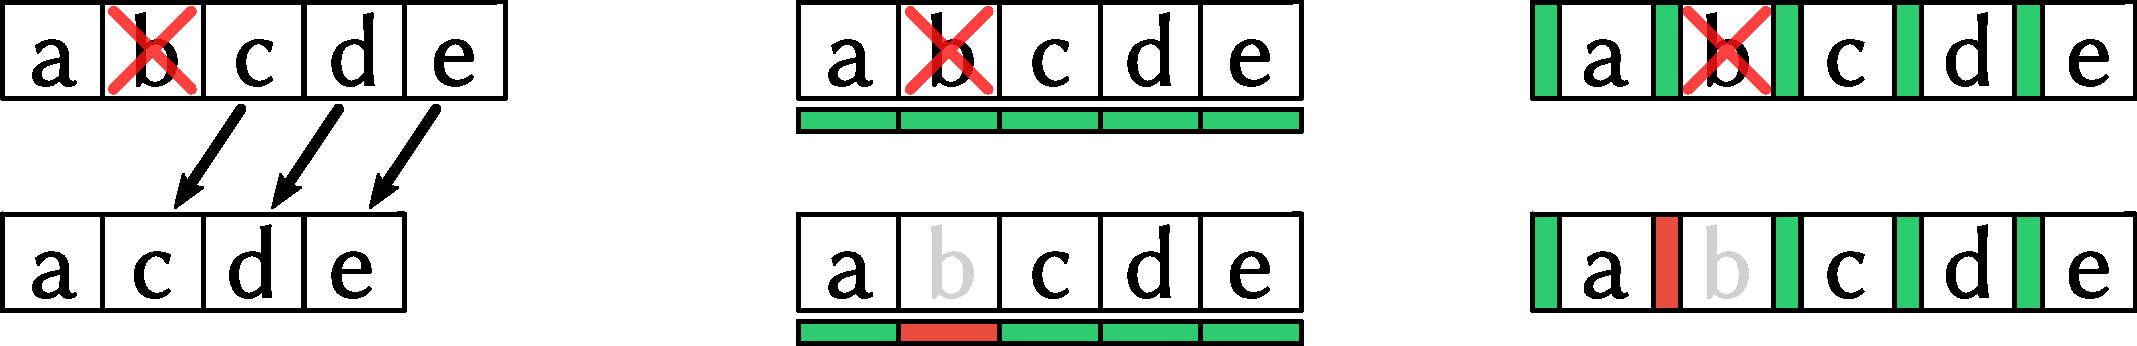
\includegraphics[width=.9\textwidth]{svg2pdf/stable-vec}
  \caption{Different ways to delete an element from a growable array: shifting elements (left), storing a \codebox{deleted} flag as a separate bit-vector (center) and storing a \codebox{deleted} flag next to the elements (right).}
  \vspace{5mm}
\end{figure}

A popular alternative way to store \code{deleted} flags is using a bit-vector, a densely packed array of bits (storing 8 bits per byte).
It has the disadvantage of requiring a separate allocation which slightly increases the reallocation cost and could potentially double the number of cache misses per element access.
However, this is usually out-weight by the benefits:
the dense packing means that no memory is wasted and that many of these flags fit into the cache at once (for example, a standard-sized L1 cache with 256~KB of storage can fit over 2~million bits, a 64~byte cache line can fit 512 bits).

It is also possible to use special \emph{sentinel values} to represent a deleted element (this is the general case of null-value optimization, where the sentinel value is 0) or to interleave the bits with the actual values in blocks to avoid an additional allocation.
A proper analysis of these different storage methods would be appropriate, but was outside the scope of this thesis.
In a quick comparison of the \code{Vec<Option<T>>} and bit-vector versions, no large difference in performance was found.
As a consequence and for memory efficiency, the bit-vector implementation was chosen for \code{lox}.
This choice is not final, however, and the implementation could easily be replaced by another one.

The logic for growable arrays that allow deletions is implemented completely independently of \code{lox} in a library called \code{stable-vec}\footnote{\url{https://crates.io/crates/stable-vec}}.
This library is technically also not part of this thesis.






\subsubsection*{Property Maps}

As mentioned in chapter 2, it is often necessary to associated arbitrary data with specific mesh elements.
This data is called \enquote{property} in this thesis; vertex normals are a \enquote{vertex property}, for example.
While some properties live as long as the mesh itself (e.\,g. vertex positions or face colors),  others are temporary values that only live for the duration of one algorithm (e.\,g. a boolean \code{visited} flag).
These temporary properties should not be kept in memory longer than necessary, meaning that they cannot be stored with the elements directly.
Instead, \code{lox} uses external maps (mapping from element to property), called \emph{property maps}.

These maps can be implemented in a variety of ways, including:

\begin{itemize}
\item A growing array using the handle ID as index (this works because it is already used as an array index in the main mesh).
\item A hash map using the handle ID as key.
\item A list of \code{(handle, value)} pairs.
\end{itemize}

In most situations, the growing array is the best choice as accessing values has virtually no overhead (apart from effects due to caching).
However, in a few situations it is necessary to associated values with only a couple of elements.
Using a growing array for that purpose is not a good idea, since the length of the array does not depend on the number of values but on the highest handle ID.
So on average, a growing array would waste a lot of memory, making other implementations a viable choice.

Just like with the mesh data structure, it does not make sense to decide on one specific implementation of external maps.
Instead, all implementations are offered by \code{lox} and abstracted over via traits.
That way, the most fitting implementation can be chosen in every situation.
The corresponding types are currently called \code{VecMap} (growable array), \code{HashMap} and \code{TinyMap} (list of tuples).
The abstraction is realized with three traits to make it as flexible as possible:

\begin{description}
  \item [\codebox{PropMap}] This trait only requires a single method to be implemented.
  Its signature is \code{fn get(&self, handle: H) -> Option<Value>} where \code{H} is the handle type parameter (this is a simplified version of the actual signature, which is explained in chapter~6).
  Returning \code{None} means that no value is associated with the given handle/element.
  This trait represents a simple map from handle to optional value.
  \item [\codebox{PropStore}] Like \code{PropMap} but can additionally iterate over all handles and values.
  \item [\codebox{PropStoreMut}] Like \code{PropStore} but can additionally change, insert and remove values.
\end{description}

The three data structures mentioned above (growing array, hash map, list of pairs) implement all three traits.
The reason for using three traits instead of a single one was to allow for more exotic type to be used.
The following types are provided by \code{lox} and implement \code{PropMap}, but not the other traits:

\begin{itemize}
\item \code{EmptyMap}: contains no properties, always returns \code{None}.
\item \code{ConstMap}: stores a single value and returns that value for all elements/handles.
\item \code{FnMap}: stores a function object with the signature \code{(&self, H) -> Option<Value>} which is used to implement \code{PropMap}.
\end{itemize}

While these types might not seem particularly useful at first, they are immensely handy in some situations.
Of course, they can be replaced by simply preparing a growable array or hash map with the desired values.
This, however, costs memory and extra time.
Specifically, \code{FnMap} is very useful to generate properties without using memory.

As a motivating example, consider an algorithm that produces a float value for each face, thus returning \code{VecMap<FaceHandle, f32>}.
This float value needs to be visualized via colors, for example by simply mapping the float value to gray-scale colors.
With \code{FnMap} a face~$\rightarrow$~color mapping can be created easily without allocating any memory:

\begin{center}
  \begin{minipage}{.59\textwidth}
    \begin{rustcode}
      let face_values = algorithm(&mesh);
      let face_colors = FnMap(|fh| {
          face_values.get(fh).map(to_color)
      });
    \end{rustcode}
  \end{minipage}
\end{center}


\subsubsection*{\enquote{Array of Structs} vs. \enquote{Struct of Arrays}}

Having property maps to store mesh properties externally brings up an interesting consideration: is it faster to use one property map per property kind or to use as few different maps as possible (e.\,g. by clustering different property kinds).
This problem is very similar to the \enquote{Array of Structs} (\emph{AoS}) vs. \enquote{Struct of Arrays} (\emph{SoA}) choice.
The two different layout strategies are visualized in figure X (TODO).

Both layouts use almost the same amount of memory and do not differ in capabilities.
The only difference is in how they interact with CPU caches.
To find an answer to what strategy should be preferred, a number of different benchmarks were conducted.


In these benchmarks, many items with a few random \code{u32} fields were stored in either one of the two memory layouts.
The time required to sum up all or some of these values was measured to get an idea of the respective speeds.
The different benchmarks attempted to cover the following parameter space:

\begin{itemize}
  \item \textbf{Memory layout}: AOS or SOA.
  \item \textbf{Traversal kind}: random or sequential.
  In the sequential benchmarks, a loop simply iterates sequentially over all indices starting from 0.
  The random benchmarks used the first field's \code{u32} value as next index to jump to.
  This was done to not include the generation of random numbers in the measured time.
  Notably, these \code{u32} values were already generated to be valid indices (i.\,e. smaller than the total number of items) and thus, the timed code does not need to perform any additional work on these values.
  \item \textbf{Total number of items}: all benchmarks were performed with 10,000, 100,000, 1,000,000 and 10,000,000 items.
  \item \textbf{Number of [used] fields per item}: 1:1, 2:1, 2:2, 4:1, 4:2, 4:4, 6:1, 6:3 and 6:6 were tested.
  The syntax X:Y means that each item has X many fields and Y many fields were included in the sum, the other fields were ignored.
\end{itemize}

The benchmark code and more details on the benchmark can be found in the repository of this thesis in the folder \code{benchmarks/memory-layout/}.
The benchmark uses the framework \emph{Criterion} \cite{criterion} which features a sophisticated statistical analysis of the raw measurements.
The actual measurement was performed on a completely idle \textsf{Thinkpad T-460p} (with an \textsf{Intel i7-6700\,HQ} running \textsf{Ubuntu 18.04}) and ran for approximately three hours.

%TODO: add and discuss results

\newpage
\section{Data Structures and Mesh Traits}

One of the main challenges in creating this library was to find a suitable set of traits that would serve as a reasonable abstraction.
A single trait is not sufficient because not all data structures offer the same set of capabilities.
On the other hand, having one trait for each individual feature of data structures (i.\,e. for each neighborhood information, each mutating operation, \dots) would result in a very large number of traits, making the library's API much harder to understand and more difficult to work with.
Finding a good solution in between those extremes is crucial for the usefulness of the abstraction.

As a first step, it is important to define what entities should be abstracted over.
As mentioned, the main goal is to be able to easily switch between different mesh data structures, which are provided by \code{lox} itself.
But users of this library can also implement the traits for their own data structures, allowing them to use many features (like mesh algorithms or IO) without \code{lox} even knowing about those types.
It can thus be beneficial to imagine what other types could reasonably implement the mesh traits.
This could include basic graph data structures, implicitly defined polygon meshes or other highly specialized data structures.
To reduce the scope of this problem, this thesis focused on known mesh data structures provided by \code{lox}.

Finding a good design for such a central interface requires knowledge about everything that interacts with it and a fair amount of experience from working with different solutions.
While quite some experience was gained during \code{lox}'s development so far, it is not sufficient to commit to one specific solution (in the opinion of the author).
Instead, a few more design iterations are to be expected.
In particular, since the library was not yet (as time of this writing) publicly released, other programmers did not have the chance to provide feedback.
This section describes the design consideration and introduces a few possible solutions.


\subsubsection*{Basic and Optional Capabilities}

A good starting point is to define the basic features of a \enquote{mesh} (the lowest common denominator) and to identify \emph{optional} capabilities.
All basic features are defined in the trait \code{Mesh} (in OOP terms: the very top of the class hierarchy).
Describing the optional capabilities (i.\,e. the features not part of \code{Mesh}) in the trait system is the main challenge in finding a good design.
Note that for now, adjacency information are ignored.

Different data structures can expose different elements in their API: faces, vertices, edge and half-edges.
Elements that are not exposed cannot be referred to and thus, associating data with those elements is not possible.
For exposed elements, we expect the data structure to be able to enumerate all elements of that kind (i.\,e. iterate over them).
As faces and vertices are needed in almost all situation and since it can be exposed by all data structures discussed so far, they are considered a basic part of meshes and are included in \code{Mesh}.
However, edges are not exposed by all data structures and are thus optional, referred to as \code{EdgeMesh} from here on.
Exposing half-edges can be useful in many situations, but are not as important as full edges.
Because of this and to reduce the scope during initial development, half-edges were ignored for the public API (of course, half-edges can still be used internally by data structures).

Another optional capability is \emph{mutability}.
Not all algorithms need to modify meshes and it is conceivable that some more exotic data structures (e.\,g. implicitly defining the mesh) do not support mutation.
As such, it makes sense to treat the ability to mutate the mesh as optional capability, called \code{MeshMut}.

The distinction between pure triangle meshes and polygon meshes also needs to be considered.
While it makes intuitive sense that polygon meshes offer an additional feature by letting algorithms create non-triangular faces, pure triangle meshes also offer additional features as some operations are only possible on triangle meshes.
So these are two mutually exclusive, optional capabilities with the extra restriction that each mesh should offer exactly one of them.
They are referred to as \code{TriMesh} and \code{PolyMesh} from here on.
(In the future, pure quad meshes will be considered in the API, too.)

Everything a mesh data structure has to offer is now in one of three categories (see figure~\ref{fig:mesh-features} for an overview):

\begin{itemize}
  \item \textbf{Basic mesh features}. For example: enumerating all vertices.
  \item \textbf{Requires \emph{one} additional capability}. For example: \code{add_vertex} (requires mutability) or enumerating all edges (requires exposed edges).
  \item \textbf{Requires \emph{multiple} additional capabilities}. For example: \code{add_face} (add face with arbitrary valence, requires mutability and \code{PolyMesh}) or \code{flip_edge} (requires mutability, \code{EdgeMesh} and \code{TriMesh}). % TODO: add figure showing edge flip
\end{itemize}

\begin{figure}[t]
  \centering
  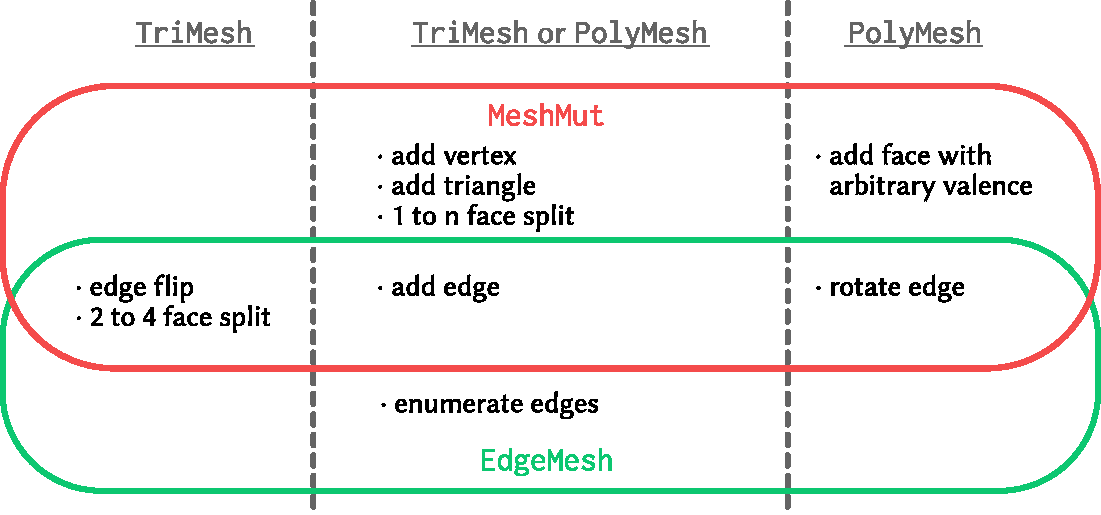
\includegraphics[width=.98\textwidth]{svg2pdf/mesh-features}
  \caption{
    A couple of example mesh features categorized by which capabilities they require (i.\,e. this diagram is not complete).
  }
  \label{fig:mesh-features}
\end{figure}

As already stated, basic mesh features are defined in \code{Mesh}.
There are multiple possibilities where all other features are defined:

\begin{itemize}
  \item Create a trait per combination of capabilities (e.\,g. \code{PolyMeshMut} for triangular meshes that can be mutated) and put each feature in the fitting trait.
  This works, but creates a large number of traits.
  Users might prefer to have functionality in as few traits as possible.
  \item Create a trait per single optional capability and put features only requiring one capability in the corresponding trait.
  Features requiring multiple capabilities are defined in the trait of one of those capabilities, defining all other capabilities by adding trait bounds to \code{Self}.
  For example, the method to add arbitrary faces could be defined in \code{MeshMut} with the following signature:

  \begin{rustcode}
    fn add_face(&mut self, vertices: &[VertexHandle]) -> FaceHandle
    where
        Self: PolyMesh;
  \end{rustcode}

  \item Like the last version, but put all methods into \code{Mesh}, completely declaring the required capabilities via bounds on \code{Self}.
  \item Some combination of the three explained possibilities.
\end{itemize}

None of these solutions is clearly better than the others which is part of the reason the design of the mesh traits is not finished yet.
The current solution is to define all methods in either \code{Mesh} or \code{MeshMut}.
Traits \code{EdgeMesh}, \code{TriMesh} and \code{PolyMesh} are added, but just serve as markers.
Methods requiring additional capabilities declare that via bounds on \code{Self}.
This design avoids having a large number of traits and all functionality is found in only two traits, making it easy to discover for users.
Also see figure~TODO.

\subsubsection*{Mutually exclusive traits}

Special attention has to be payed to the design of \code{TriMesh} and \code{PolyMesh}.
Simply adding two traits would be incorrect, because types could implement neither or both of these traits which should be prohibited.
To solve this problem, the trait \code{Mesh} could declare an \emph{associated constant} and the two traits could be defined in terms of this constant:

\begin{rustcode}
  enum FaceKind { Triangle, Polygon }

  trait Mesh {
      const FACE_KIND: FaceKind;
  }

  trait TriMesh: Mesh<FACE_KIND = FaceKind::Triangle> {}
  trait PolyMesh: Mesh<FACE_KIND = FaceKind::Polygon> {}

  // Blanket implementation to automatically implement traits for all types
  // that also implement Mesh with the correct face kind.
  impl<T: Mesh<FACE_KIND = FaceKind::Triangle> TriMesh for T {}
  impl<T: Mesh<FACE_KIND = FaceKind::Polygon> PolyMesh for T {}
\end{rustcode}

Implementors need to define a value for the constant when implementing the trait.
\code{TriMesh} and \code{PolyMesh} are automatically implemented for these types implementing \code{Mesh} with the corresponding value set.
The only problem with this approach is that it does not compile yet:
the Rust compiler still lacks the ability to check value equality within trait bounds.
Luckily, this problem can simply be worked around by using types instead of values and using an associated type instead of an associated constant.

\begin{rustcode}
  // Two types instead of two values.
  enum TriFace {}
  enum PolyFace {}

  // A trait which is only implemented for these types (not strictly
  // necessary, but avoids misuse of the API).
  trait FaceKind {}
  impl FaceKind for TriFace {}
  impl FaceKind for PolyFace {}

  trait Mesh {
      type FaceKind: FaceKind;  // Type instead of constant
  }

  trait TriMesh: Mesh<FaceKind = TriFace> {}
  trait PolyMesh: Mesh<FaceKind = PolyFace> {}

  // Blanket implementation to automatically implement traits for all types
  // that also implement Mesh with the correct face kind.
  impl<T: Mesh<FaceKind = TriFace> TriMesh for T {}
  impl<T: Mesh<FaceKind = PolyFace> PolyMesh for T {}
\end{rustcode}


\subsubsection*{Adjacency Traits}

All functionality regarding adjacency information has to be defined in traits as well which has much the same design considerations.
Defining too many traits (e.\,g. one trait per basic adjacency query) would make the whole API more confusing while a single trait would not be flexible enough.
The current design consists of three traits:

\begin{itemize}
  \item \textbf{\codebox{BasicAdj}}: this trait only defines \adj{F}{V} adjacency.
  This is arguably the most used neighborhood query as it is needed for basic rendering and IO.
  The trait is implemented by all mesh data structures within \code{lox}.
  \item \textbf{\codebox{FullAdj}}: requires \code{BasicAdj} and adds \adj{F}{F}, \adj{V}{F} and \adj{V}{V} queries, meaning that all queries between faces and vertices are supported.
  It is implemented by all data structures except for \code{SharedVertexMesh}.
  \item \textbf{\codebox{EdgeAdj}}: requires \code{BasicAdj} and adds \adj{E}{F}, \adj{E}{V}, \adj{F}{E} and \adj{V}{E}.
  This is currently only implemented by \code{HalfEdgeMesh}.
\end{itemize}

This solution works fairly well for mesh data structures defined within \code{lox}, but has not been evaluated for potential external data structures:
The main advantage is the low number of traits which simplifies the API.
But as mentioned above, this design is likely to change in the future.

Figure~\ref{fig:mesh-traits} shows an overview of all currently existing traits.

\begin{figure}[th]
  \centering
  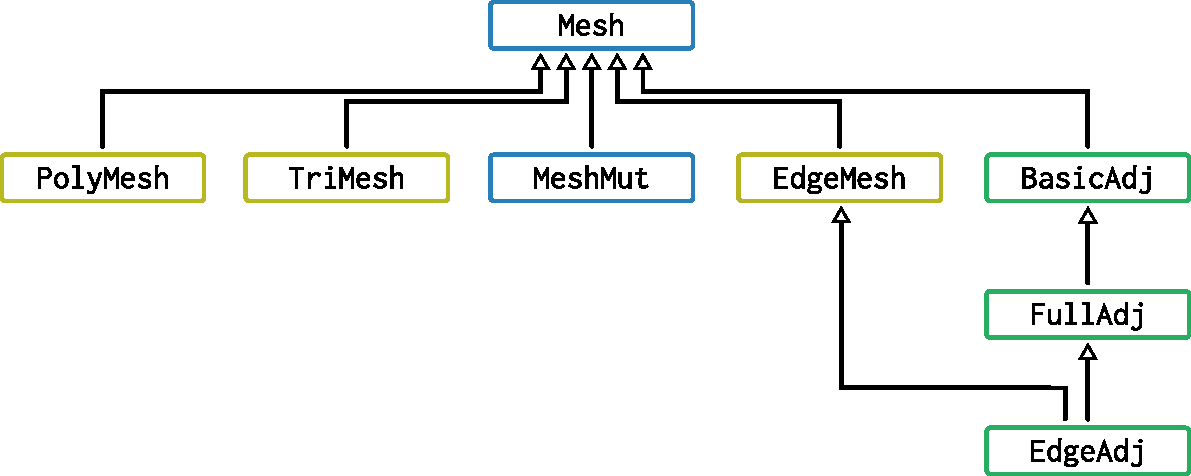
\includegraphics[width=.98\textwidth]{svg2pdf/mesh-traits}
  \caption{
    Traits currently used in \codebox{lox} to abstract over meshes.
    The arrows represents \emph{super trait bounds}, i.\,e. \codebox{Mesh} is a super trait of \codebox{MeshMut}.
    Green boxes contain traits that deal with adjacency information, yellow boxes indicate marker traits without own methods.
  }
  \label{fig:mesh-traits}
\end{figure}




\newpage
\section{Input/Output Module}


\section{Optimizations}


\section{Overview of all Library Features}
